\chapter{通信网的可靠性}
\section{可靠性理论概要
}
\subsection{不可修复系统的可靠度
}
所谓不可修复系统是该系统一旦启用,直到损坏或失效为止,一旦失效,就不会再回到运行状态。
这种系统只有两个状态:\textbf{一为运行,另一为失效;而且只有运行状态向失效状态转移一种可能。}\\
\subsubsection{理论分析}
定义可靠度:
\begin{equation}\label{key}
R(t) = P[\text{工作时间}>t] = P[t\text{t时刻仍正常工作}],R[0] = 1
\end{equation}
定义不可靠度:
\begin{equation}\label{key}
F(t) = 1 - R(t) =P[\text{工作时间}>t] =  P[\text{t时刻不能正常工作}]
\end{equation}
故障率,失效率(平均)$ \alpha $
\begin{equation}\label{key}
dt\text{失效的概率} = \alpha dt
\end{equation}
\begin{figure}[H]
	\centering
	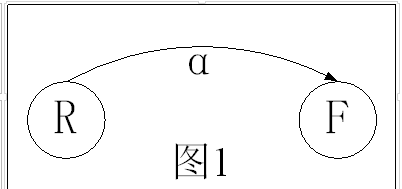
\includegraphics[width=0.7\linewidth]{figures/screenshot085}
	\caption{}
	\label{fig:screenshot085}
\end{figure}

\textbf{t时刻正常,经$ \Delta t $还没有失效有:$ R(t+\Delta t)=R(t) ·(1-a\Delta t) $
},解一个微分方程即可。
求得:
\begin{equation}\label{key}
R(t) = e^{-at}
\end{equation}
所以
\begin{equation}\label{key}
F(t) = 1-R(t) = 1-e^{-at}
\end{equation}
因此寿命t的概率密度函数$ f(t) $为:
\begin{equation}\label{key}
f(t) = F^{'}(t) = -R^{'}(t) = \alpha R(t)
\end{equation}
平均寿命:
\begin{equation}\label{key}
T  = \int_{0}^{\infty} R(t) dt = \int_{0}^{\infty} e^{-\alpha t} dt = \frac{1}{\alpha}
\end{equation}


\begin{figure}[H]
	\centering
	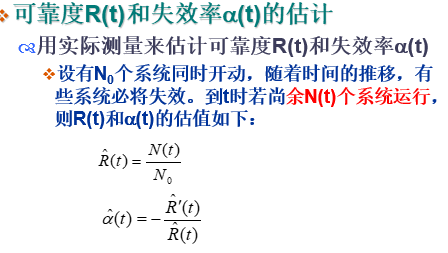
\includegraphics[width=0.7\linewidth]{figures/screenshot086}
	\caption{}
	\label{fig:screenshot086}
\end{figure}
\subsubsection{寿命分析}
\begin{figure}[H]
	\centering
	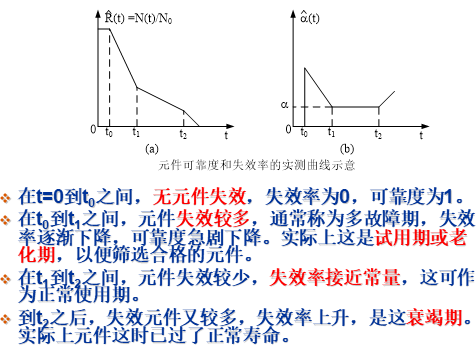
\includegraphics[width=0.7\linewidth]{figures/screenshot087}
	\caption{}
	\label{fig:screenshot087}
\end{figure}


\subsection{可修复系统的可靠度}
对于大型设备,不能一出故障就丢弃,而是要把它\textbf{修复再使用},这类系统称为可修复系统。此时,不但能从\textbf{正常运行状态转移到失效状态},而且还能从\textbf{失效状态转移到正常运行状态}。
前者仍可用失效率a来表示转移概率;后者可相仿地定义修复率b。
\begin{figure}[H]
	\centering
	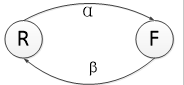
\includegraphics[width=0.4\linewidth]{figures/screenshot088}
	\caption{}
	\label{fig:screenshot088}
\end{figure}
当在t时处于失效状态的条件下,\textbf{在$ t $到$ t+dt $内修复的概率为$ \beta dt $}。
\begin{figure}[H]
	\centering
	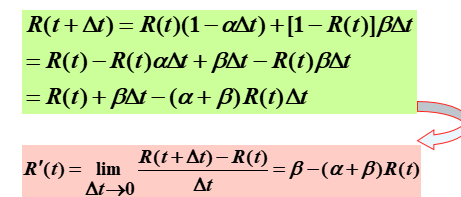
\includegraphics[width=0.7\linewidth]{figures/screenshot089}
	\caption{}
	\label{fig:screenshot089}
\end{figure}
求解上述微分方程:
\begin{figure}[H]
	\centering
	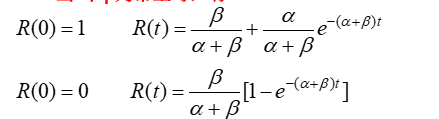
\includegraphics[width=0.7\linewidth]{figures/screenshot090}
	\caption{}
	\label{fig:screenshot090}
\end{figure}
t$ -> \infty$时
\begin{equation}\label{key}
R(t) = \frac{\beta}{\alpha+\beta}
\end{equation}
\begin{description}
	\item[MTBF] Mean Time Between Failures
	\begin{equation}\label{key}
	MTBF = \frac{1}{\alpha}
	\end{equation}
	\item[MTTR] Mean Time To Repair
	\begin{equation}\label{key}
	MTTR = \frac{1}{\beta}
	\end{equation}
\end{description}
\begin{equation}\label{key}
R(t) = \frac{MTBF}{MTBF+MTTR} = \frac{\beta}{\alpha+\beta}
\end{equation}

\subsection{复杂系统的分解
}
\subsubsection{串接系统}
\begin{gather}\label{key}
R = \varPi_{r = 1}^{n}R_r\\
F = 1-R = 1- \varPi_{r = 1}^{n}R_r
\end{gather}
\textbf{如果是n个不可修复系统},则系统可靠度为
\begin{equation}\label{key}
R = e^{-nat}
\end{equation}
寿命为
\begin{equation}\label{key}
T= \frac{1}{na}
\end{equation}
若各子系统的\textbf{可靠度相差悬殊},则作为近似计算,高可靠度的失效率较小,可以忽略不计。也就是计算总的可靠度或平均寿命,常\textbf{只选几个薄弱环节},亦即几个低可靠度的子系统来计算,这样可简化。\\
\vspace{2pt}
\textbf{如果是n个独立可修复系统}:
\begin{figure}[H]
	\centering
	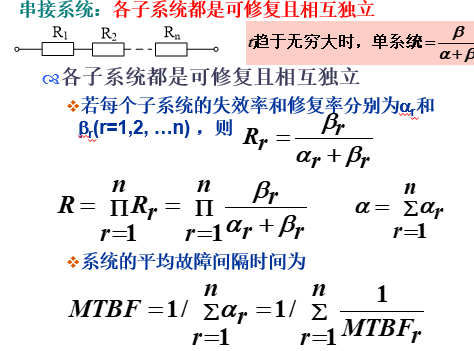
\includegraphics[width=0.7\linewidth]{figures/screenshot091}
	\caption{}
	\label{fig:screenshot091}
\end{figure}
\begin{figure}[H]
	\centering
	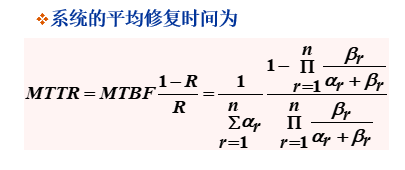
\includegraphics[width=0.7\linewidth]{figures/screenshot092}
	\caption{}
	\label{fig:screenshot092}
\end{figure}
\textbf{如果是n个非独立可修复系统}:
\begin{figure}[H]
	\centering
	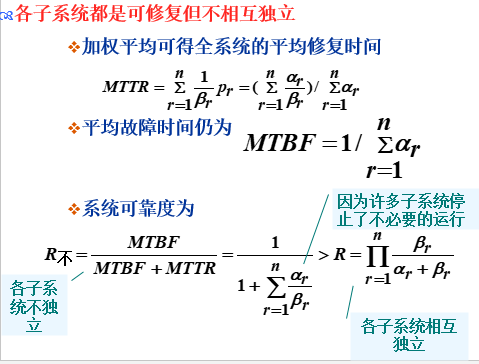
\includegraphics[width=0.7\linewidth]{figures/screenshot093}
	\caption{}
	\label{fig:screenshot093}
\end{figure}
\textbf{子系统中有可修复系统和不可修复系统:}
则整个系统的平均寿命为:
\begin{equation}\label{key}
R=T_{\text{不可修复}}R_{\text{可修复}}
\end{equation}
\begin{figure}[H]
	\centering
	
\includegraphics[width=0.7\linewidth]{figures/screenshot094}
	\caption{}
	\label{fig:screenshot094}
\end{figure}
\subsubsection{并接系统}
\begin{gather}\label{key}
F = \varPi_{r = 1}^{n}F_r = \varPi_{r = 1}^{n} (1-R_r)\\
R= 1-F = 1- \varPi_{r = 1}^{n} (1-R_r)
\end{gather}
\begin{figure}[H]
	\centering
	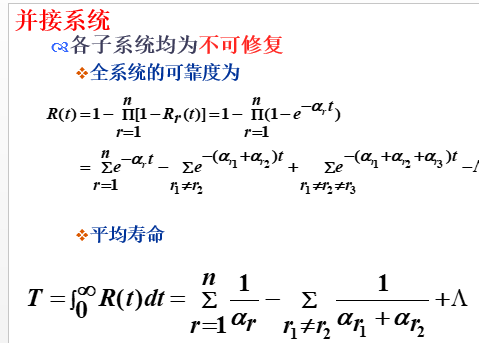
\includegraphics[width=0.7\linewidth]{figures/screenshot095}
	\caption{}
	\label{fig:screenshot095}
\end{figure}
\begin{figure}[H]
	\centering
	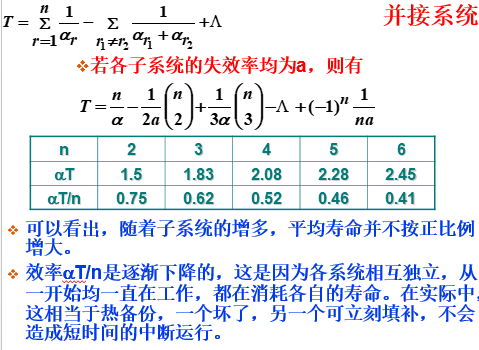
\includegraphics[width=0.7\linewidth]{figures/screenshot096}
	\caption{}
	\label{fig:screenshot096}
\end{figure}
上述过程为热备份。\\
冷备份(旁置备份):某个时间段内只开启一个系统,只有当这个系统故障了才开启另一个,这会造成启动时间差。\\
半热备份,一个子系统在运行,另一个处于半工作状态,如预热。\\
寿命对比:
\[
T_\text{冷} > T_\text{半热} >T_\text{热} 
\]
列写状态转移时,出为负,进为正。
\begin{figure}[H]
	\centering
	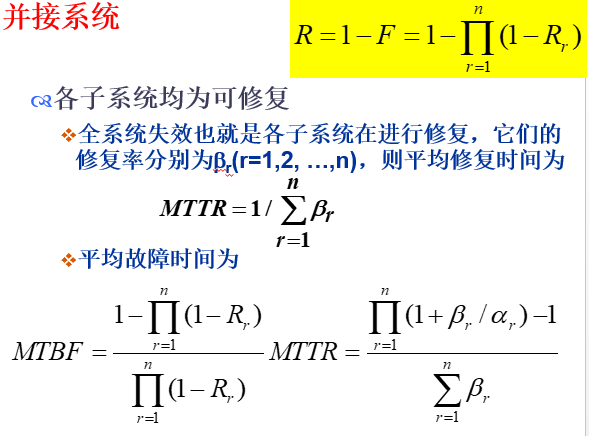
\includegraphics[width=0.7\linewidth]{figures/screenshot097}
	\caption{}
	\label{fig:screenshot097}
\end{figure}
\subsection{串并混合}
\subsection{桥式电路}

\begin{figure}[H]
	\centering
	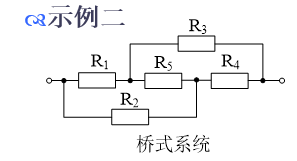
\includegraphics[width=0.7\linewidth]{figures/screenshot098}
	\caption{}
	\label{fig:screenshot098}
\end{figure}
\begin{figure}[H]
	\centering
	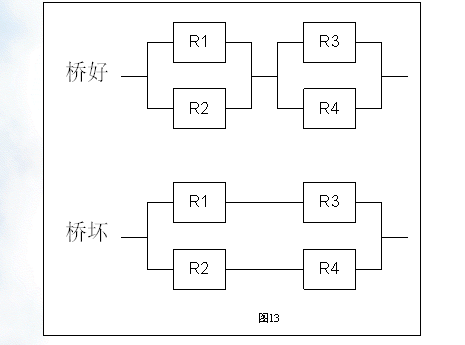
\includegraphics[width=0.7\linewidth]{figures/screenshot099}
	\caption{}
	\label{fig:screenshot099}
\end{figure}
\begin{figure}[H]
	\centering
	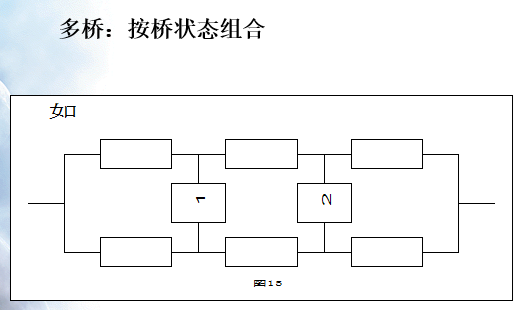
\includegraphics[width=0.7\linewidth]{figures/screenshot100}
	\caption{}
	\label{fig:screenshot100}
\end{figure}
\begin{figure}[H]
	\centering
	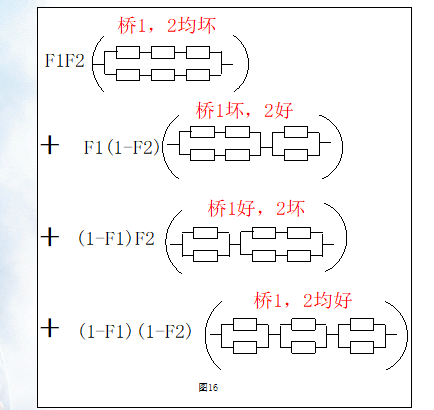
\includegraphics[width=0.7\linewidth]{figures/screenshot101}
	\caption{}
	\label{fig:screenshot101}
\end{figure}


\subsection{可靠性设计
}
\begin{itemize}
	\item 避免串接的子系统过多
	\item 必要时采用备份以形成并接系统
	\item 尽量减小各子系统或部件的故障率
	\item 尽量增加修复率
\end{itemize}
\begin{figure}[H]
	\centering
	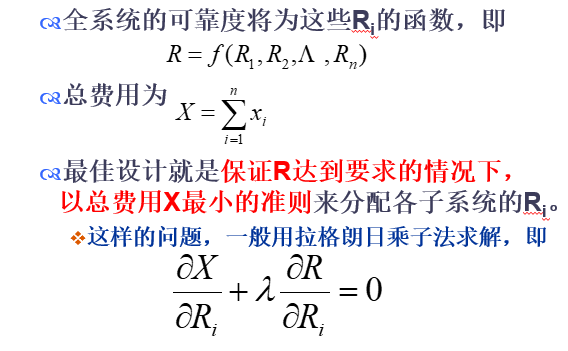
\includegraphics[width=0.7\linewidth]{figures/screenshot102}
	\caption{}
	\label{fig:screenshot102}
\end{figure}

\section{通信网的可靠性}
\begin{enumerate}
	\item 第1种定义是从整个网出发,图可能成为不联结的,那么从整体上说,网已失效。
	\item 着眼于网内某些端
	\item 从随机图出发,设代表网的图并不是确定的,任两端之间有边与否是以概率规定。
\end{enumerate}

\section{通信网的联结性
}
\begin{itemize}
	\item $ \alpha $最小割端集的端数
	\item $ \beta $最小割边集的边数,当各端度数相等时,可使$ \beta $等于$ 2m/n $。正则图
	\item $ \gamma $上述的混合
	\item $ 2m/n $,冗余度
\end{itemize}
\begin{equation}\label{key}
\gamma = \alpha \le \beta \le 2m/n
\end{equation}
边数最小的连接图为树,中的任两端之间只有一条径,去掉一条边或一个端,必使图成为不联结的。

\section{局间通信和综合可靠度
}

